%!TEX root = CSL.tex

We now turn to the study of modalities in the classical setting, focusing on the positive-negative modal logic \PNL\ with nominals \cite{DBLP:journals/jolli/XiongA20,DBLP:journals/logcom/PedersenSA21}. This logic is based on Kripke frames with two disjoint and symmetric reachability relations. In these notes we will outline the construction of an adequate semantic game for \PNL, its transformation into a provability game, and the derivation of a corresponding sequent system. This opens a discussion of how to escalate this method to other modal systems.

We begin with a brief discussion of games for modal logics and the motivation for hybrid extensions. As studied in~\cite{blackburn-synthese} and further developed in~\cite{Robert-PhD}, extending Lorenzen-style~\cite{Lorenzen1978-LORDLJ-2} dialogue game to modal logic is conceptually straightforward: in addition to the current roles of the players and the current formula $F$, one only has to  keep track of the current world $w$ in the model. However, this extension introduces an unfortunate drawback: the {\em game trees}, \ie, labelled trees whose nodes are game states, are no longer determined solely by the syntax of the formula, but instead depend on the relational structure of the model. This is in stark contrast to semantic games for propositional logic, where semantic information is required only at the final stage to determine the winner. The loss of uniformity in game trees across all models is a significant limitation of this approach.

As in~\cite{blackburn-synthese,DBLP:conf/wollic/Freiman21}, we address this problem by turning to hybrid logic~\cite{DBLP:journals/jolli/BlackburnS95,DBLP:journals/japll/BraunerP06,brauner2010hybrid}, allowing explicit references to worlds and the accessibility relation within the object language. 

Let $\A=\{\ag,\b,\ldots\}$ be a non-empty set of agents,
$\At=\{p,q,\ldots\}$ be a countable set of propositional variables, and $N=\{i,j,\ldots\}$ be a countable set of \emph{nominals}. The language of \PNL~is generated by the following grammar
$$F  ::= p  \mid \neg F  \mid F_1  \wedge F_2  \mid F_1  \vee F_2  \mid  R^+(i,j)\mid R^-(i,j) \mid  \dplus F  \mid \dminus F \mid [A]F $$
where $p\in \At$, and $i,j\in N$.  Formulas of the form $p$, $R^+(i,j)$, or $R^-(i,j)$ are called \emph{elementary}. We shall use $F,G,H$ to range over formulas. 
The propositional connectives $\top$, $\bot$, $\to$, and the (dual)  modalities $\bplus$ and $\bminus$ can be obtained in the usual way. 

 Intuitively, nominals are used as names for worlds of the model, while the propositions $R^\pm(i,j)$ state that agent $i$ is a  \emph{friend}/\emph{enemy} with
 $j$. 
The formula $\dplus F $ (resp. $\dminus F $) states that $F $ holds for  a friend (resp.\ an enemy). The global
modality $[A]F $ states that $F $ holds for all the agents. 
We use $R^\pm$ to denote either $R^+$ or $R^-$, and 
 $\dplusminus$ to denote either $\dplus$ or $\dminus$. 

A model $\mathbb{M}$ is a tuple $\langle \A,\R^+,\R^-,\V,\g\rangle$ where $\A$
is a set (of agents), $\g:N\rightarrow \A$ is called \emph{denotation
function}, $\R^+,\R^-\subseteq \A\times \A$, and $\V:\At\rightarrow
\mathcal{P}(\A)$. 
%
A model is a \PNL-model if:
\begin{itemize}
\item $\g$ is surjective, \ie, every agent has a name;
\item $\R^+$ is reflexive; and
\item $\R^+$ and $\R^-$ are both symmetric and 
non-overlapping, \ie,  for all $\ag,\b\in \A$, $(\ag,\b)\notin \R^+$ or $(\ag,\b)\notin \R^-$. 
\end{itemize}  
The Kripke semantics of \PNL~is in \Cref{fig:ksem}.
A formula $F$ is true over $\mathbb{M}$, written $\mathbb{M}\Vdash F$ iff
$\mathbb{M},\ag\Vdash F$, for all agent $\ag\in\A$. For a set of formulas
$\Delta$, we write $\mathbb{M}\models \Delta$ iff $\mathbb{M}\Vdash \Delta$ for all $F
\in \Delta$. A formula $F$ is valid iff $\mathbb{M}\Vdash F$ for every
\PNL-model $\mathbb{M}$. For a class of models $\mathfrak{M}$, we write
$\Delta\models_{\mathfrak{M}} F$ iff $\mathbb{M}\Vdash F$ for every model
$\mathbb{M}\in \mathfrak{M}$ with $\mathbb{M}\models \Delta$. 


\begin{figure}
$\small
\qquad\begin{array}{lll l lll}
    \mathbb{M},\ag \Vdash p &\text{ iff } \ag\in \V(p) &\quad& 
    \mathbb{M},\ag \Vdash \neg F &\text{ iff } \mathbb{M},\ag \not \Vdash F\\
    \mathbb{M},\ag \Vdash F \wedge G &\text{ iff } \mathbb{M},\ag \Vdash F \text{ and } \mathbb{M},\ag \Vdash G &\quad&
    \mathbb{M},\ag \Vdash F \vee G &\text{ iff } \mathbb{M},\ag \Vdash F \text{ or } \mathbb{M},\ag \Vdash G\\
    \mathbb{M},\ag \Vdash R^\pm(i,j) &\text{ iff } (\g(i),\g(j))\in \R^\pm\\
    \mathbb{M},\ag \Vdash \dplusminus F &\multicolumn{6}{l}{\text{ iff there is } j\in N \text{ such that } \mathbb{M},\g(j)\Vdash R^{\pm}(i,j)  \text{ and } \mathbb{M},\g(j)\Vdash  F }\\
    \mathbb{M},\ag \Vdash [A] F  &\multicolumn{6}{l}{\text{ iff } \mathbb{M},\g(j)\Vdash  F , \text{ for all } j\in N.}
\end{array}
$
\caption{Kripke semantics for \PNL\label{fig:ksem}.}
\end{figure}

\begin{example}
Consider the following models (omitting self loops for $\R^+$):
\begin{center}



\tikzset{every picture/.style={line width=0.75pt}} %set default line width to 0.75pt        

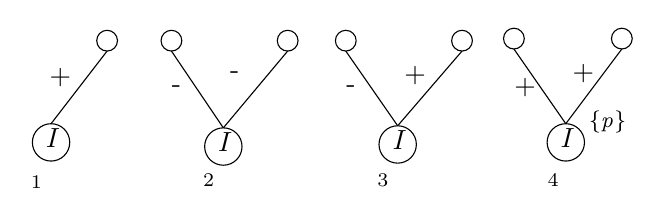
\begin{tikzpicture}[x=0.75pt,y=0.75pt,yscale=-1,xscale=1]
%uncomment if require: \path (0,300); %set diagram left start at 0, and has height of 300

%Shape: Circle [id:dp45081245928280866] 
\draw   (35,99) .. controls (35,94.03) and (39.03,90) .. (44,90) .. controls (48.97,90) and (53,94.03) .. (53,99) .. controls (53,103.97) and (48.97,108) .. (44,108) .. controls (39.03,108) and (35,103.97) .. (35,99) -- cycle ;
%Straight Lines [id:da3823547043352371] 
\draw    (44,90) -- (71,55) ;
%Shape: Circle [id:dp19703461573841063] 
\draw   (66,50) .. controls (66,47.24) and (68.24,45) .. (71,45) .. controls (73.76,45) and (76,47.24) .. (76,50) .. controls (76,52.76) and (73.76,55) .. (71,55) .. controls (68.24,55) and (66,52.76) .. (66,50) -- cycle ;
%Straight Lines [id:da4683229017954724] 
\draw    (127,92) -- (158,55) ;
%Shape: Circle [id:dp2867759515585031] 
\draw   (153,50) .. controls (153,47.24) and (155.24,45) .. (158,45) .. controls (160.76,45) and (163,47.24) .. (163,50) .. controls (163,52.76) and (160.76,55) .. (158,55) .. controls (155.24,55) and (153,52.76) .. (153,50) -- cycle ;
%Straight Lines [id:da5314947280596498] 
\draw    (127,92) -- (102,55) ;
%Shape: Circle [id:dp1959928048918531] 
\draw   (97,50) .. controls (97,47.24) and (99.24,45) .. (102,45) .. controls (104.76,45) and (107,47.24) .. (107,50) .. controls (107,52.76) and (104.76,55) .. (102,55) .. controls (99.24,55) and (97,52.76) .. (97,50) -- cycle ;
%Straight Lines [id:da4112188353179198] 
\draw    (211,91) -- (242,55) ;
%Shape: Circle [id:dp42913203090443486] 
\draw   (237,50) .. controls (237,47.24) and (239.24,45) .. (242,45) .. controls (244.76,45) and (247,47.24) .. (247,50) .. controls (247,52.76) and (244.76,55) .. (242,55) .. controls (239.24,55) and (237,52.76) .. (237,50) -- cycle ;
%Straight Lines [id:da043439872331601403] 
\draw    (211,91) -- (186,55) ;
%Shape: Circle [id:dp8295578596165345] 
\draw   (181,50) .. controls (181,47.24) and (183.24,45) .. (186,45) .. controls (188.76,45) and (191,47.24) .. (191,50) .. controls (191,52.76) and (188.76,55) .. (186,55) .. controls (183.24,55) and (181,52.76) .. (181,50) -- cycle ;
%Straight Lines [id:da6496682295510845] 
\draw    (292,90) -- (319,54) ;
%Shape: Circle [id:dp5439224913830538] 
\draw   (314,49) .. controls (314,46.24) and (316.24,44) .. (319,44) .. controls (321.76,44) and (324,46.24) .. (324,49) .. controls (324,51.76) and (321.76,54) .. (319,54) .. controls (316.24,54) and (314,51.76) .. (314,49) -- cycle ;
%Straight Lines [id:da2985458825783045] 
\draw    (292,90) -- (267,54) ;
%Shape: Circle [id:dp5841558365361761] 
\draw   (262,49) .. controls (262,46.24) and (264.24,44) .. (267,44) .. controls (269.76,44) and (272,46.24) .. (272,49) .. controls (272,51.76) and (269.76,54) .. (267,54) .. controls (264.24,54) and (262,51.76) .. (262,49) -- cycle ;
%Shape: Circle [id:dp9925510753878242] 
\draw   (118,101) .. controls (118,96.03) and (122.03,92) .. (127,92) .. controls (131.97,92) and (136,96.03) .. (136,101) .. controls (136,105.97) and (131.97,110) .. (127,110) .. controls (122.03,110) and (118,105.97) .. (118,101) -- cycle ;
%Shape: Circle [id:dp3643673494287285] 
\draw   (202,100) .. controls (202,95.03) and (206.03,91) .. (211,91) .. controls (215.97,91) and (220,95.03) .. (220,100) .. controls (220,104.97) and (215.97,109) .. (211,109) .. controls (206.03,109) and (202,104.97) .. (202,100) -- cycle ;
%Shape: Circle [id:dp13429278332775496] 
\draw   (283,99) .. controls (283,94.03) and (287.03,90) .. (292,90) .. controls (296.97,90) and (301,94.03) .. (301,99) .. controls (301,103.97) and (296.97,108) .. (292,108) .. controls (287.03,108) and (283,103.97) .. (283,99) -- cycle ;

% Text Node
\draw (40,91) node [anchor=north west][inner sep=0.75pt]   [align=left] {\textit{I}};
% Text Node
\draw (42,62) node [anchor=north west][inner sep=0.75pt]   [align=left] {+};
% Text Node
\draw (33,114) node [anchor=north west][inner sep=0.75pt]   [align=left] {$\M_1$};
% Text Node
\draw (129,61) node [anchor=north west][inner sep=0.75pt]   [align=left] {\mbox{-}};
% Text Node
\draw (116,113) node [anchor=north west][inner sep=0.75pt]   [align=left] {$\M_2$};
% Text Node
\draw (101,68) node [anchor=north west][inner sep=0.75pt]   [align=left] {\mbox{-}};
% Text Node
\draw (213,61) node [anchor=north west][inner sep=0.75pt]   [align=left] {+};
% Text Node
\draw (200,113) node [anchor=north west][inner sep=0.75pt]   [align=left] {$\M_3$};
% Text Node
\draw (185,68) node [anchor=north west][inner sep=0.75pt]   [align=left] {\mbox{-}};
% Text Node
\draw (294,60) node [anchor=north west][inner sep=0.75pt]   [align=left] {+};
% Text Node
\draw (282,113) node [anchor=north west][inner sep=0.75pt]   [align=left] {$\M_4$};
% Text Node
\draw (266,67) node [anchor=north west][inner sep=0.75pt]   [align=left] {+};
% Text Node
\draw (302,82.5) node [anchor=north west][inner sep=0.75pt]   [align=left] {{\footnotesize \{\textit{p}\}}};
% Text Node
\draw (123,93) node [anchor=north west][inner sep=0.75pt]   [align=left] {\textit{I}};
% Text Node
\draw (207,92) node [anchor=north west][inner sep=0.75pt]   [align=left] {\textit{I}};
% Text Node
\draw (288,91) node [anchor=north west][inner sep=0.75pt]   [align=left] {\textit{I}};


\end{tikzpicture}

\end{center}
The following hold:
\begin{itemize}
\item[$\M_1$] $I$ have a friend: $\M_1, I \Vdash \dplus\top$;
\item[$\M_2$] $I$ do not have friends: $\M_2, I \Vdash \bplus\bot$;
\item[$\M_3$] $I$ have a friend and an enemy: $\M_3, I \Vdash \dplus \top\,\wedge \dminus\top$;
\item[$\M_4$] Everybody has a friend where $p$: $\M_4, \ag \Vdash  [A ]  \dplus p$ for any agent $\ag$.
\end{itemize} 
 \end{example}


\subsection{Playing with models}\label{sec:game-semantics}
Before starting playing, remember that in a \PNL-model $\M$, every agent $\ag$ has a name $i$, \ie, there exists $i\in N$ s.t. $\g(i)=\ag$. Hence, from now on, we will internalise the nominals, identifying an agent $\ag$ with its respective nominal $i$.

The  \emph{semantic game} is played over a \PNL-model $\M=(\A,\R^+,\R^-,\V,\g)$ by two
players, \Me (or \Ic) and \You, who argue about the truth of a formula $ F $ at an
agent $i$. At each stage of the game, one player acts as \emph{proponent}, while the
other acts as \emph{opponent} of the claim that  $ F $ is true at 
$i$. 

We represent the situation where \Ic am the proponent (and \You are the
opponent) by the \emph{game state} $\mathbf{P}, i: F $, and the situation
where \Ic am the opponent (and \You are the proponent) by $\mathbf{O},
i: F $. 

We call a game state \emph{elementary} if its involved formula is elementary. For a game state $g$, we denote the game starting at $g$ over the model $\M$ by $\mathbf{G}_\M(g)$.

The game over a \PNL-model $\M$ proceeds by reducing the involved formula $ F $ to an elementary formula by following the rules described in Figure~\ref{fig:game-rules}.


\begin{figure}
~~~\resizebox{.92\textwidth}{!}{
\begin{minipage}[t]{\textwidth}
    \hrulefill
\begin{description}
\item[$(\mathbf{P}_\wedge)$] At $\mathbf{P},  i :  F _1\wedge  F _2$, \You
    choose between  $\mathbf{P}, i : F _1$ and 
    $\mathbf{P}, i : F _2$ to continue the game. \\
\item[$(\mathbf{O}_\wedge)$] \vspace{-2mm}At $\mathbf{O},  i :
     F _1\wedge  F _2$, \Ic choose between $\mathbf{O}, i : F _1$
    and $\mathbf{O}, i : F _2$ to continue the game. \\

\item[$(\mathbf{P}_\vee)$] At $\mathbf{P},  i :  F _1\vee  F _2$, \Ic choose between $\mathbf{P}, i : F _1$ and $\mathbf{P}, i : F _2$ to continue the game.\\
\item[$(\mathbf{O}_\vee)$] \vspace{-2mm}At $\mathbf{O},  i :  F _1\vee  F _2$, \You choose between $\mathbf{O}, i : F _1$ and $\mathbf{O}, i : F _2$ to continue the game.\\

\item[$(\mathbf{P}_\neg)$] At $\mathbf{P},  i : \neg  F $, the game continues with $\mathbf{O},  i :  F $.\\
\item[$(\mathbf{O}_\neg)$] \vspace{-2mm}At $\mathbf{O},  i : \neg  F $, the game continues with $\mathbf{P}, i :  F $.\\
    \item[$(\mathbf{P}_{\Diamond^\pm})$] At $\mathbf{P}, i: \Diamond^\pm  F $, \Ic choose a nominal $j$, and \You decide whether the game ends in the state $\mathbf{P},\_:R^\pm(i,j)$ or continues with $\mathbf{P},j:  F $.\\
        \item[$(\mathbf{O}_{\Diamond^\pm})$] \vspace{-2mm} At $\mathbf{O},i: \Diamond^\pm  F $, \You choose  $j$, and \Ic choose between $\mathbf{O},\_:R^\pm(i,j)$ and $\mathbf{O},j: F $.\\
\item[$(\mathbf{P}_{[A]})$] At $\mathbf{P},i: [A] F $, \You choose a nominal $j$ and the game continues with $\mathbf{P},j: F $.\\
\item[$(\mathbf{O}_{[A]})$] \vspace{-2mm} At $\mathbf{O},i: [A] F $, \Ic choose a nominal $j$, and the game continues with $\mathbf{O},j:  F $.\\
\item[$(\mathbf{P}_{el})$] Let $ F _{e}$ be an elementary formula. \Ic win and \You lose at $\mathbf{P}, i : F _{e}$ iff $~\mathbb{M}, i  \models  F _{e}$. Otherwise, \You win and \Ic lose.\\
\item[$(\mathbf{O}_{el})$] \vspace{-2mm}At $\mathbf{O}, i  :  F _{e}$, \Ic win and \You lose iff $\mathbb{M}, i \not \models  F _{e}$. Otherwise, \You win and \Ic lose.\\
\end{description}
    \hrulefill
\end{minipage}
}
\caption{Semantic game given a \PNL-model $\M$.\label{fig:game-rules}}
\end{figure}

In general, every two-person, zero-sum, win-lose game is usually represented by
a game tree. In our
case, the root of the game tree representing the game
$\mathbf{G}_\mathbb{M}(g)$ is $g$. The children of each node in the game tree
are exactly the possible choices of the corresponding player. For instance, if
$h=\mathbf{P},  i :  F _1\wedge  F _2$ appears in the game tree, then its
children are $\mathbf{P}, i : F _1$ and $\mathbf{P}, i : F _2$. Each node in
the tree is labelled either ``I'', or ``Y'', depending on which player is to
move in the corresponding game state, and we label 
the nodes  $\mathbf{P},  i : \neg  F $ and $\mathbf{O},  i :
\neg  F $ with ``I'' (even though there is no choice involved in these game
states). For instance, the node corresponding to the game state $h$ above is
``Y'', since it is \Your choice in $\mathbf{P}: F _1\wedge  F _2$. The leaves
of the tree receive the label of the winning player. 
A \emph{run} of the game is a maximal path through the game tree.

Now we are ready to define winning strategies and state the main result of this section:
the adequacy of the proposed game semantics with respect to the Kripke semantics for \PNL.

\begin{definition}
    A \emph{strategy} for \Me in the game $\mathbf{G}_\M(g)$ is a subtree $\sigma$ of the associated game tree such that: 
 \textbf{(1)} $g\in \sigma$,
 \textbf{(2)} if $h\in \sigma$ is a node labeled ``Y'', then all children of $h$ are in $\sigma$,
 \textbf{(3)} if $h\in \sigma$ is a node labeled ``I'', then exactly one child of $h$ is in $\sigma$.
The strategy $\sigma$ is called \emph{winning} if all leaves in the tree $\sigma$ are labeled ``I''. (Winning) strategies for \You are defined dually.
\end{definition}

\begin{theorem}[Adequacy - semantic games~\cite{LPAR2024:Reasoning_About_Group_Polarization}]%\label{winningstrategy}
\label{th:adequacy}
Let $\M$ be a \PNL-model, $\ag$ an agent with nominal $i$, and $F$ a formula.

\noindent\textbf{(1)} \Ic have a winning strategy for $\mathbf{G}_\M(\mathbf{P}, i:F)$ iff $\M,\ag \models F$. 

\noindent\textbf{(2)} \You have a winning strategy for $\mathbf{G}_{\M}(\mathbf{P}, i:F)$ iff $\M,\ag\not \models F$.
\end{theorem}

 
  \begin{example}[\cite{LPAR2024:Reasoning_About_Group_Polarization}]\label{ex:balance}
     Let 
     $ \mathbf{(4B)} = 
        ((\dplus\dplus p \vee \dminus\dminus p)\to \dplus p) \wedge
        ((\dplus \dminus p \vee \dminus\dplus p)\to \dminus p)
    $. This formulas 
    specifies \emph{local balance} \cite{DBLP:journals/logcom/PedersenSA21}
    and   captures the idea that 
``the enemy of my enemy is my friend'',  ``the friend
of my enemy is my enemy'',  and ``the friend of my friend is my friend''.
 A collectively connected network where $[A]4B$ holds is a polarized network, 
where agents can be divided into two opposing groups \cite{balance}.
Notions such a weak-balance \cite{weak-balance} can be also formalized in \PNL~\cite{DBLP:journals/logcom/PedersenSA21}.
    $\Ic$ have a winning strategy for the game $\bfP,\ag : 4B$
    on $\bbM_1$ 
    while $\You$ have a winning strategy for the same game on $\bbM_2$ where (omitting self-loops for $\R^+$):

	\vspace{0,4cm}
    \begin{tabularx}{.6\textwidth}{ X X X X X }
        $\bbM_1=$ & \parbox[c]{\hsize}{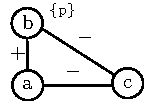
\includegraphics[scale=0.85]{fig2}} & \qquad &
        $\bbM_2=$ & \parbox[c]{\hsize}{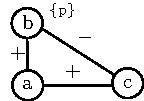
\includegraphics[scale=0.85]{fig3}} 
    \end{tabularx}

	\vspace{0,4cm}
    For $\bbM_1$, in the first conjunct, \Ic pick ($\bfP_\vee$)
    $\dplus p$ and then $\b$ in ($\bfP_{\dplus}$); for the second conjunct,
    \Ic pick the first disjunction in $F=(\dplus \dminus p \vee \dminus\dplus p)\to \dminus p)$
    where, in any of \Your choices ($\bfP_{\neg}$ followed by $\bfO_{\vee}$ and 
    $\bfO_{\Diamond^{\pm}}$), \Ic  win all the elementary states. 
    For $\bbM_2$, \Ic do not have a winning strategy 
    for the  second conjunct: \Ic can neither win $\dminus p$ (no $\R^{-}$ successor), 
    nor the first disjunct in  $F$ above since, after $\bfP_{\neg}$, 
    \You choose  ($\bfO_{\vee}$) 
    $\dplus\dminus p$ and select $\mathsf{c}$ and then $\b$ ($\bfO_{\Diamond^{\pm}}$)
    where $p$ holds and \You win. See the complete game in our tool \cite{tool}. 
	%\todo{Appendix}
% and \Cref{ap:examples}.
\end{example}

\subsection{Playing all models}
We now elevate semantic games to a \PNL-provability games. The key observation is that the rules of the semantic game remain independent of the underlying model, except at the level of elementary game states.

The {\em provability game}
$\mathbf{DG}(\mathbf{P},i:F )$ can be thought of as \Me and \You playing all
semantic games $\mathbf{G}(\mathbf{P},i:F )$ over all \PNL-models $\M$
simultaneously. We point out that  the rules of the semantic game do not depend on the structure
of $\M$ but merely on $F $. Truth degrees are only needed at the atomic level
to determine who wins the particular run of the game. This allows us to require
players to play ``blindly'', \ie, without explicitly referencing  a model $\M$.
Clearly, if \Ic have a winning strategy in such a game, then \Ic can win in
$\mathbf{G}_\M(\mathbf{P},i:F )$, for every $\M$, making this strategy an
adequate witness of logical validity. 

Provability game states are finite multisets of the game states
defined in Section \ref{sec:game-semantics}. We denote by $g_1 \bigvee ... \bigvee g_n$ 
 the provability game state $\{g_1,...,g_n\}$.
% , but keep the convenient notation $g\in D$ if $g$ is in the  multiset $D$. 
We write $D_1 \bigvee D_2$ for the
multiset sum $D_1+D_2$ and $D\bigvee g$ for $D+\{g\}$. A provability state is
called \emph{elementary} if all its game states are elementary.
We use $\mathbf{DG}(D)$ to denote the provability game starting at $D$. 

\begin{definition}\label{def:win}
Let $D^{el}$ denote the provability state consisting of the elementary game
states of $D$. \Ic win and \You lose at $D$ if for every \PNL-model there is
a game state in $D^{el}$ where \Ic win the corresponding semantic game. 
\end{definition}

In the provability game, \Ic additionally take the
role of a \emph{scheduler}, deciding which game  is to be played next. We
signal the chosen game state by underlining it as in $\underline{g}$.


\begin{figure}
\resizebox{0.93\textwidth}{!}{
\begin{minipage}[t]{\textwidth}
\hrulefill
\begin{description}
%\item[(End)] If no state in $D$ is underlined, \Ic can end the game and $D$ becomes terminal.
\item[(Dupl)] If no state in $D$ is underlined,
    %and $D$ is not terminal, 
    \Ic can choose a non-elementary $g\in D$ and the game continues with $D\bigvee g$.
\item[(Sched)] If no state in $D=D'\bigvee g$ is underlined,
    %and $D$ is not terminal, 
    and $g$ is non-elementary, 
    \Ic can choose to continue the game  with $D'\bigvee \underline{g}$.
\item[(Move)] If $D=D'\bigvee \underline{g}$ then the player who is to move in
    the semantic game $\mathbf{G}(g)$ at $g$ makes a legal move to the game
    state $g'$ and the game continues with $D' \bigvee g'$.
\item[(End)]
    The game ends if there are no non-elementary game states left in $D$, or if
    no game state is underlined and \Ic win according to
    Definition~\ref{def:win}. Otherwise, \Ic must move according to
    \textbf{(Dupl)} or \textbf{(Sched)}.
\end{description}
\hrulefill
\end{minipage}
}
\caption{Rules for the provability game\label{fig:dg-rules}.}
\end{figure}

\begin{definition}\label{def:dg}
    The rules of the provability game are in \Cref{fig:dg-rules}.
%\noindent %Additionally, we require that if no game state of $D$ is underlined, \Ic must move according to 
%\textbf{(End)}, 
%\textbf{(Dupl)} or \textbf{(Sched)}. \textbf{(Dupl)} is referred to as the \emph{duplication rule} and \textbf{(Sched)} as the \emph{scheduling}, or \emph{underlining rule}.
Infinite runs, and runs that end in elementary provability states where \Ic do not win according to Definition~\ref{def:win}, are winning for \You and losing for \Me.  \textbf{(Dupl)} is referred to as the \emph{duplication rule} and \textbf{(Sched)} as the \emph{scheduling}, or \emph{underlining rule}.
\end{definition}

\begin{theorem}[Adequacy - provability games~\cite{LPAR2024:Reasoning_About_Group_Polarization}]
\label{thm:adeq} \Ic have a winning strategy in $\mathbf{DG}(D)$  iff for every  \PNL-model $\mathbb{M}$, there is some $g\in D$ such that \Ic have a winning strategy in $\mathbf{G}_\mathbb{M}(g)$.
\end{theorem}

\begin{corollary}
The formula $F $ is  \PNL-valid iff \Ic have a winning strategy in $\mathbf{DG}(\mathbf{P},i:[A]F )$.
\end{corollary}

\begin{example}
Consider  the game $\mathbf{P},i: p \vee \neg p$.
\Ic duplicate the game state in the first round and the
game continues with the provability state $\mathbf{P},i: p \vee \neg
p\bigvee \mathbf{P},i: p \vee \neg p$. 

Now \Ic move to $\mathbf{P},i: p$ in the
first subgame and to $\mathbf{P},i:\neg p$ in the second. After a role switch
in the second subgame, the final state is $\mathbf{P},i: p \bigvee
\mathbf{O},i: p$, where \Ic win regardless of the underlying model.
\end{example}

\subsection{From games to proofs}\label{sec:proofs}

Theorems~\ref{th:adequacy} and \ref{thm:adeq} establish that winning strategies for \Me in the provability game correspond to the validity of formulas. In this section, we extend this result to proof systems by introducing a sequent calculus, 
$\DS$, where proofs correspond to \My's winning strategies in the provability game.

{\em Labeled nominal formulas} are either \emph{labeled formulas} of
the form $i: F $ or \emph{relational atoms} of the form $R(i,j)$,
where $i$ and $j$ are nominals and $ F $ is a \PNL~formula.%
\footnote{Observe that here we are abusing the notation, identifying $k:R(i,j)$ with $R(i,j)$.} \emph{Labeled sequents} have the form $\Gamma \seq \Delta$, where
$\Gamma,\Delta$ are multisets containing labeled nominal formulas.

Starting with sequents, every provability state of the form
\begin{center}
$
\mathbf{O},i_1:  F_1\bigvee \ldots \bigvee \mathbf{O},i_n:  F_n\bigvee\mathbf{P},j_1: G_1 \bigvee \ldots \bigvee \mathbf{P},j_m: G_m
$
\end{center}
 can be rewritten as the labeled sequent $\Gamma \seq \Delta$ where
$
\Gamma =\{i_1: F_1, \ldots, i_n: F_n\}\mbox{ and } \Delta =\{j_1: G_i,\ldots,j_m: G_m\}
$. 
In what follows, we will not distinguish between provability states and their corresponding labeled sequent. For example,
the provability game state
$\mathbf{O},i:(\dplus\dplus p \vee \dminus\dminus p)\bigvee\mathbf{P},i: \dplus p$
will be identified with the sequent  
$i:(\dplus\dplus p \vee \dminus\dminus p)\seq i: \dplus p$.

The inference rules must be tailored in such a way that {\em
proofs} in the sequent system match exactly \My\  {\em winning strategies} in
the provability game. This means that the user of the proof system takes the
role of \Me, scheduling game states and choosing moves in \I-states. 
Moreover, {\em provability} in the proof system should correspond to {\em
validity} in the game. For that,  it is necessary to establish the
formal relationship between elementary game states and logical axioms.


\begin{lemma}\label{lemma:init}
    Let $\Gamma\seq \Delta$ be composed of elementary game states only. \Ic win the provability game in $\Gamma \seq \Delta$ iff one of the following holds\footnote{\label{foot:sym}Since relations are symmetric, we will identify $R^\pm(i,j)$ with  $R^\pm(j,i)$.} 
%\begin{itemize}
    
    \noindent\textbf{i.} $R^-(i,i)\in\Gamma$ or $R^+(i,i)\in\Delta$ for some $i$;

    \noindent\textbf{ii.} $\{R^+(i,j),R^-(i,j)\}\subseteq\Gamma$ for some $i\not=j$;

    \noindent\textbf{iii.} $\Gamma\cap\Delta\not=\emptyset$.
\end{lemma}

\begin{comment}
Observe that the models are 
\begin{itemize}
\item [-] non overlapping: if $(\g(i),\g(j))\in \R^{\pm}$, thus by definition if $R^\pm(i,j)\in \Gamma$, then by 
$\neg$(ii) $R^\mp(i,j)\notin \Gamma$, %, and by  $\neg$(iii)  $R^\pm(i,j)\not\in \Delta$. 
hence $(\g(i),\g(j))\notin \R^{\mp}$.
\item[-] $\R^-$"-irreflexivity: $\neg$(i) implies that $(\g(i),\g(i))\notin \R^{-}$;
\item[-] in the case of collectively connectedness, we complete $\mathbb{M}$ as follows: for all $R^\pm(i,j)\in\Delta$, 
add $(\g(i),\g(j))\in \R^{\mp}$; and for all remaining nominals $k,l$ appearing in $\Gamma\seq\Delta$ such that $R^\pm(k,l)\notin \Gamma,\Delta$, add $(\g(k),\g(l))\in \R^{+}$. Observe that $\neg(iii)$ plus 
 $\neg$(iv) guarantee the non-overlapping. 
\end{itemize}
In both cases, the defined models are such that  \You win in $g$ over $\M$, whenever $g\in D$.
\end{comment}

Figure~\ref{fig:calculus} presents the labeled sequent systems $\DS$ with the standard initial axiom and structural/propositional  rules. The modal  rules and the relational rules $sym$ and  $ref\pm$  coincides with the modal rules originally presented by Vigan\`{o} in~\cite{Vigano:2000}, adapted to multi-relational modal logics. 
%
It is routine to show that the rule $no$ in Figure~\ref{fig:calculus} correspond to the non-overlapping  axiom
$
\forall i,j. \neg(R^+(i,j)\wedge R^-(i,j)) 
$.

The following result immediately implies that the provability game $\mathbf{DG}$ is adequate with respect to the calculus $\DS$.

\begin{theorem}[Adequacy - sequent system~\cite{LPAR2024:Reasoning_About_Group_Polarization}]\label{thm:adequacy-sequent}
\Ic have a winning strategy in the provability game $\mathbf{DG}(\Gamma\seq\Delta)$  iff $\Gamma\seq\Delta$ is provable in $\DS$. 
\end{theorem}

Let us write $\models_\PNL \Gamma \Rightarrow \Delta$ iff for every \PNL-model there is some $i:F \in \Gamma$ such that $\M,\g(i)\not\vdash F$, or there is some $i:G \in \Delta$ such that $\M,\g(i)\models G$. We have the following consequence of Theorems~\ref{th:adequacy},~\ref{thm:adeq}, and~\ref{thm:adequacy-sequent}: 

\begin{corollary}
Let $\Gamma,\Delta$ be multisets of labeled formulas. Then $\models_\PNL\Gamma \Rightarrow \Delta$ iff there is a proof of $\Gamma \Rightarrow \Delta$ in $\DS$. In particular, $ F $ is \PNL-valid iff there is a proof of $\Rightarrow  F $ in $\DS$.
\end{corollary}

\begin{figure}[ht]
    \begin{center}
\resizebox{.85\textwidth}{!}{
\begin{minipage}[t]{\textwidth}
	\headline{\sc Axiom and Structural Rules}
	
	\medskip

    \begin{center}
 \begin{prooftree}
        \hypo {}
        \infer1 [$init$]{\Gamma, i: F_{el} \Rightarrow  \Delta, i: F_{el}}
        \end{prooftree}
\qquad
 \begin{prooftree}
        \hypo {\Gamma, i:  F, i:  F  \Rightarrow  \Delta}
        \infer1 [$(L_c)$]{\Gamma, i:  F  \Rightarrow  \Delta}
        \end{prooftree}        
		\qquad
        \begin{prooftree}
        \hypo {\Gamma \Rightarrow  i:  F ,i:  F ,\Delta}
        \infer1 [$(R_c)$]{\Gamma \Rightarrow  i:  F , \Delta}
        \end{prooftree}
    \end{center}
        
\headline{\sc Propositional Rules}
\begin{center}
        \begin{prooftree}
        \hypo {\Gamma \Rightarrow i:  F , \Delta}
        \infer1 [\((L_\neg)\)]{\Gamma, i: \neg  F  \Rightarrow \Delta}
        \end{prooftree}
  \qquad
  \begin{prooftree}
        \hypo {\Gamma, i:   F  \Rightarrow \Delta}
        \infer1[\((R_\neg)\)]{\Gamma \Rightarrow i: \neg   F , \Delta}
        \end{prooftree}

\bigskip

        \begin{prooftree}
        \hypo {\Gamma, i:  F  \Rightarrow \Delta}
        \hypo{\Gamma, i: G \Rightarrow \Delta}
        \infer2 [\((L_\vee)\)]{\Gamma, i:  F  \vee  G \Rightarrow \Delta}
        \end{prooftree}
        \qquad
        \begin{prooftree}
        \hypo {\Gamma \Rightarrow i:   F , \Delta}
        \infer1[\((R_\vee^1)\)]{\Gamma \Rightarrow i:   F  \vee  G, \Delta}
        \end{prooftree}
        \qquad 
        \begin{prooftree}
        \hypo {\Gamma \Rightarrow i:  G, \Delta}
        \infer1[\((R_\vee^2)\)]{\Gamma \Rightarrow i:   F  \vee  G, \Delta}
        \end{prooftree}
        \bigskip

        \begin{prooftree}
        \hypo {\Gamma, i:  F  \Rightarrow \Delta}
        \infer1 [\((L_\wedge^1)\)]{\Gamma, i:  F  \wedge  G \Rightarrow \Delta}
        \end{prooftree}
       \qquad
    	\begin{prooftree}
        \hypo {\Gamma, i: G \Rightarrow \Delta}
        \infer1 [\((L_\wedge^2)\)]{\Gamma, i:  F  \wedge  G \Rightarrow \Delta}
        \end{prooftree}
       \qquad
       \begin{prooftree}
        \hypo {\Gamma \Rightarrow i:   F , \Delta}
        \hypo {\Gamma \Rightarrow i:  G, \Delta}
        \infer2[\((R_\wedge)\)]{\Gamma \Rightarrow i:   F  \wedge  G, \Delta}
        \end{prooftree}
                
    \end{center}
\headline{\sc Modal Rules}
\begin{center}
         \begin{prooftree}
        \hypo {\Gamma, R^\pm(i,j) \Rightarrow \Delta}
        \infer1 [\((L_{\Diamond^\pm})_1\)]{\Gamma, i: \Diamond^\pm  F \Rightarrow \Delta}
        \end{prooftree}
       \qquad
       \begin{prooftree}
        \hypo {\Gamma, j: F  \Rightarrow \Delta}  
        \infer1 [\((L_{\Diamond^\pm})_2\)]{\Gamma, i: \Diamond^\pm  F \Rightarrow \Delta}
        \end{prooftree}
      \bigskip
      
      \begin{prooftree}
        \hypo {\Gamma \Rightarrow R^\pm(i,j), \Delta}
        \hypo {\Gamma \Rightarrow j:  F , \Delta}
        \infer2 [\((R_{\Diamond^\pm})\)]{\Gamma\Rightarrow i: \Diamond^\pm  F ,\Delta}
        \end{prooftree}
        \quad
        \begin{prooftree}
        \hypo {\Gamma, j:  F  \Rightarrow \Delta}
        \infer1 [$(L_{[A]})$]{\Gamma,  i:[A] F  \Rightarrow \Delta}
        \end{prooftree}
        \quad
        \begin{prooftree}
        \hypo {\Gamma \Rightarrow  j:  F , \Delta}
        \infer1 [$(R_{[A]})$]{\Gamma\Rightarrow  i:[A] F , \Delta}
        \end{prooftree}

    \end{center}

        
\headline{\sc Relational Rules}
\begin{center}
         \begin{prooftree}
        \hypo {\Gamma \Rightarrow  \Delta, R^{\pm}(j,i)}
        \infer1 [$sym$]{\Gamma \Rightarrow  \Delta, R^{\pm}(i,j)}
        \end{prooftree}
        \qquad
\begin{prooftree}
        \hypo { }
        \infer1 [$ref+$]{\Gamma\Rightarrow  \Delta, R^{+}(i,i)}
        \end{prooftree}
        \bigskip

\begin{prooftree}
        \hypo { }
        \infer1 [$ref-$]{\Gamma, R^{-}(i,i)\Rightarrow  \Delta}
        \end{prooftree}
        \qquad
        \begin{prooftree}
        \hypo {\Gamma \Rightarrow  \Delta, R^+(i,j)}
        \hypo {\Gamma \Rightarrow  \Delta, R^-(i,j)}
        \infer2 [$no$]{\Gamma \Rightarrow  \Delta}
        \end{prooftree}
    \end{center}
        
\end{minipage}
}
\end{center}
\vspace{-0.3cm}
%        \begin{prooftree}
%        \hypo {\Gamma, R^+(i,j) \Rightarrow  \Delta}
%        \hypo {\Gamma, R^-(i,j) \Rightarrow  \Delta}
%        \infer2 [$cc$]{\Gamma \Rightarrow  \Delta}
%        \end{prooftree}
 \caption{The proof system $\DS$.
     %is formed by the initial axiom plus the structural, propositional, relational and modal rules.  
     In the rule init, $F_{el}$ denotes an
elementary formula. In the rules   $(L_{\Diamond^\pm})_1$,
$(L_{\Diamond^\pm})_2$, and $(R_{[A]})$,  the nominal $j$ is fresh.% (this condition corresponds to \emph{Your} optimal choice). 
The rule
$R_{\meddiamondminus}$ has the proviso that $i\neq j$.  \label{fig:calculus} } 
\end{figure}

Proving cut-admissibility of labeled systems can be cumbersome due to the presence of relational rules. %(see \eg\ \cite{negri99aml}).
%Moreover, it is usually done in a case-by-case analysis, tailored for each system (see \eg\ \cite{negri99aml}). 
%
In~\cite{DBLP:journals/apal/MarinMPV22}, a systematic procedure for
transforming axioms into rules was presented, based on {\em focusing} and {\em
polarities}~\cite{andreoli92jlc}. This procedure not only allows for 
generalizing different approaches for transforming axioms into sequent
rules present in the literature~\cite{Sim94,Vigano:2000,Neg05}, but it also provides 
a uniform way of proving cut-admissibility for the resulting systems.

The cut-admissibility result for $\DS$ is a particular instance of the general result in~\cite{DBLP:journals/apal/MarinMPV22}.
\begin{theorem}[\PNL-cut]\label{thm:cut}
The following cut rule is admissible in $\DS$

\vspace{0.15cm}
\qquad\qquad\qquad\qquad$
\infer[cut]{\Gamma\seq\Delta}{\Gamma\seq\Delta,i: F  & i: F ,\Gamma\seq\Delta}
$
\end{theorem}
%For the reader interested in understanding focusing, polarities and the axioms-as-rules approach, we have added a gentle introduction in Appendix~\ref{app:focusing}. We refer to~\cite{DBLP:journals/apal/MarinMPV22} for further reading on the topic.
As a consequence, %of Theorem~\ref{thm:cut}, 
$\DS/\DS$ are consistent, since the only rules that can be applied in an empty sequent is $no$ and it is routine to show that it does not trivialize derivations. 



